\begin{figure}[] \centering
	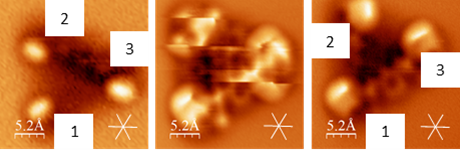
\includegraphics[width=0.7\textwidth]{./images/hbbnc-ag-111-leg-flip}
	\caption{Conformational change of a HBBNC monomer after several scans with the AFM. First the molecule starts with an orientation of the legs in 1: clockwise, 2: counterclockwise, 3: clockwise. After several scans in close proximity legs at positions 2 and 3 flip around and change their orientation to 1: clockwise, 2: clockwise, 3: counterclockwise. This results in a changed adsorption geometry. First the upper right edge is lifted from the substrate, while after the leg rearrangement the lower right edge is lifted from the surface. This is caused by the lower lying dimethyl groups lifting the phenyl ring and the molecule's edge connected to it.}
	\label{fig:HBBNC-nc-AFM-legs-change}
\end{figure}

\begin{figure}[] \centering
	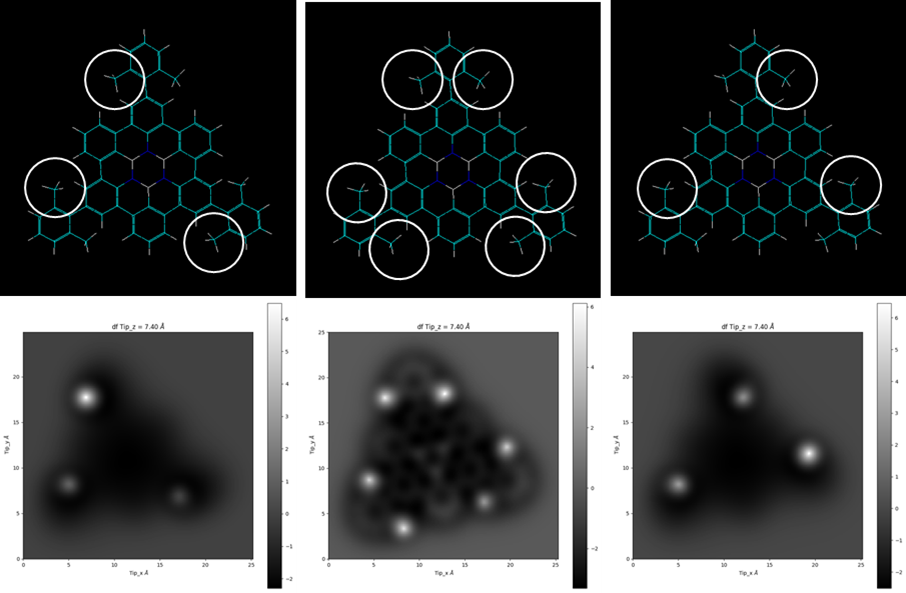
\includegraphics[width=0.7\textwidth]{./images/Simulated-AFM-flipping-legs}
	\caption{Calculated AFM images for freestanding HBBNC. The coronene has been aligned to lie flat in the image plane. Three different leg rotations are shown. The highest features are enclosed by white circles. In the middle column, all phenyl rings are parallel to  the image plane, resulting in six features in the calculated image above the dimethyl groups. Columns to the left/right show AFM images as would be expected by a rotation of the dimethylphenyl rings by $\pm \SI{20}{\degree}$. The rotation direction is chosen as described in \autoref{fig:HBBNC-nc-AFM-legs-change} and reproduces the highest appearing spots in the AFM images well. The used code was published as web tool \cite{_AFM_calc} and bases on  \cite{hapala_origin_2014,hapala_mechanism_2014}.}
	\label{fig:HBBNC-nc-AFM-legs-change-calc}
\end{figure}


\begin{figure}[] \centering
	\subfigure[Variable height simulated AFM images for type I connection.]{
		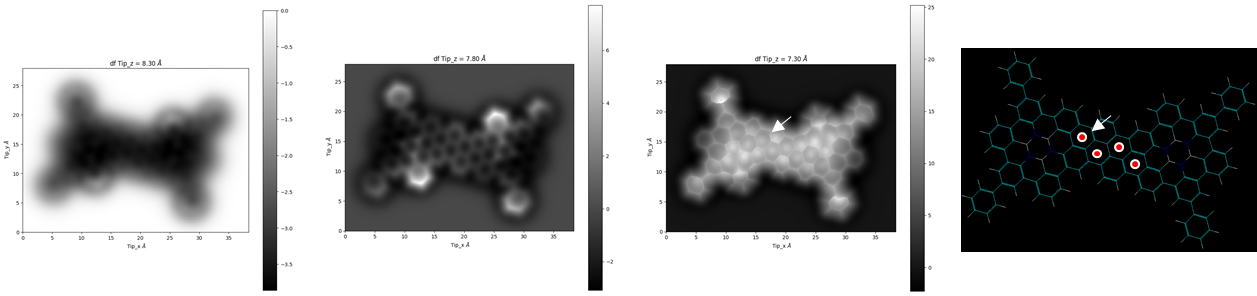
\includegraphics[width=\textwidth]{./images/hbbnc-planar-ring-structure-lost-methyl}
		\label{fig:HBBNC-planar-ring-1}
	}
	\subfigure[]{
		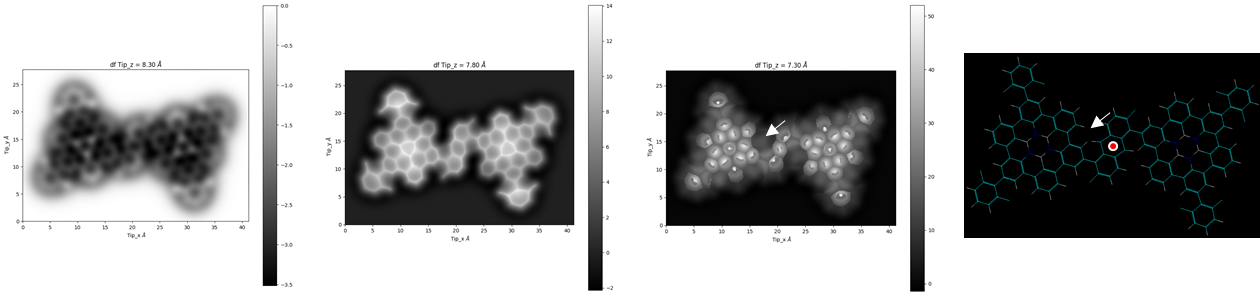
\includegraphics[width=\textwidth]{./images/hbbnc-planar-ring-structure-link2}
		\label{fig:HBBNC-planar-ring-2}
	}
	\caption{Simulated AFM images showing the change in structure of a dimer formed by two different binding motifs as explained in \autoref{fig:HBBNC-linking}. Calculated AFM images given for three different heights. An arrow is placed next to spots where experimental identification between the two types is difficult and requires best tip conditions. New features visible in AFM are highlighted by a dot in the molecular model.}
	\label{fig:HBBNC-ring-structure}
\end{figure}

\begin{figure}[] \centering
	\subfigure[HBBNC before...]{
		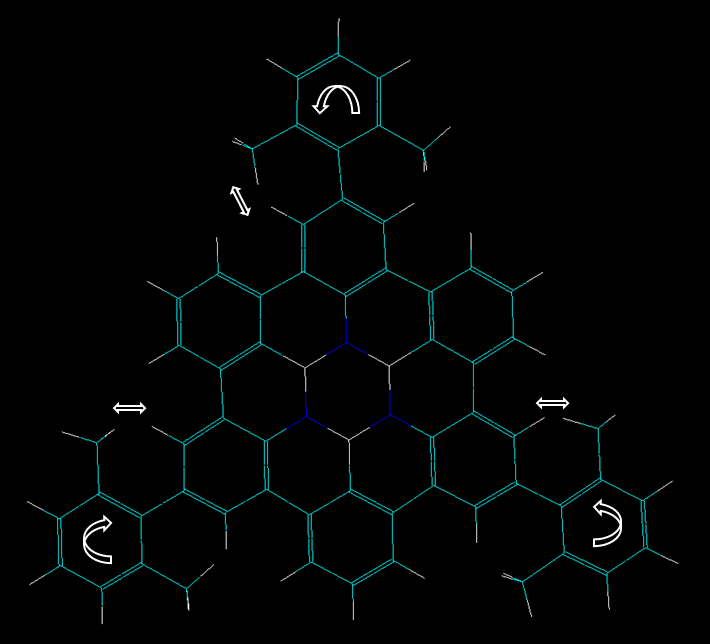
\includegraphics[width=0.45\textwidth]{./images/B3LYP-relaxed-flat-legs}
		\label{fig:HBBNC-B3LYP-relaxed-flat-legs}
	}
	\subfigure[...and after ring closure reaction.]{
		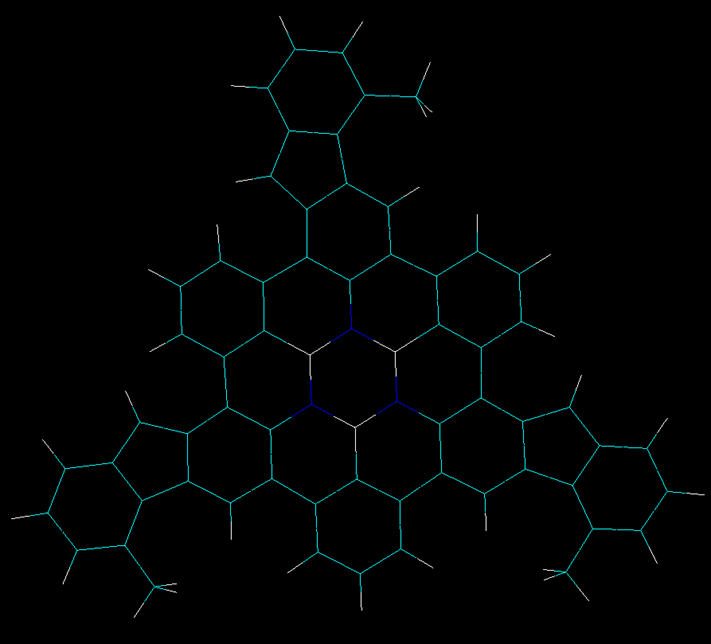
\includegraphics[width=0.45\textwidth]{./images/B3LYP-relaxed-fixed-core-rings-closed}
		\label{fig:HBBNC-B3LYP-relaxed-fixed-core-rings-closed}
	}
	\caption{Possible ring closure reaction after annealing HBBNC. \subref{fig:HBBNC-B3LYP-relaxed-flat-legs} In HBBNC the upper and right leg are rotated counterclockwise and the methyl group links with the coronene body. This creates a new 5-membered ring and bends the leg. A connection with opposing direction (clockwise) is present for the left leg. \subref{fig:HBBNC-B3LYP-relaxed-fixed-core-rings-closed} Depending on the turn direction of the di-methyl-phenyl leg, two turn directions of the modified leg funtionalization form. 
	}
	\label{fig:HBBNC-ring-closure}
\end{figure}

\begin{figure}[] \centering
	\subfigure[]{
		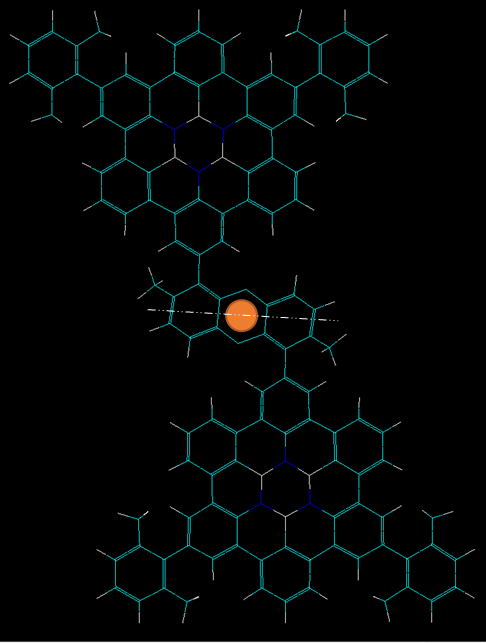
\includegraphics[height=0.35\textwidth]{./images/AM1-methyl-groups-fuse-link-2-split-hydrogen-mod}
		\label{fig:HBBNC-AM1-methyl-groups-fuse-link-2-split hydrogen}
	}
	\subfigure[]{
		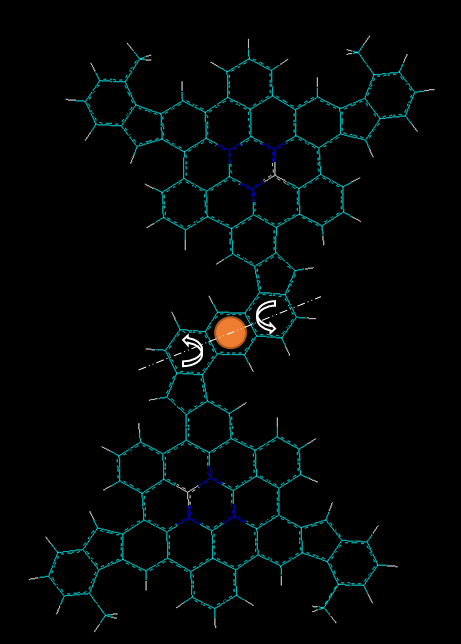
\includegraphics[height=0.35\textwidth]{./images/Closed-ring-dimer-1}
		\label{fig:HBBNC-Closed-ring-dimer-1}
	}
	\subfigure[]{
	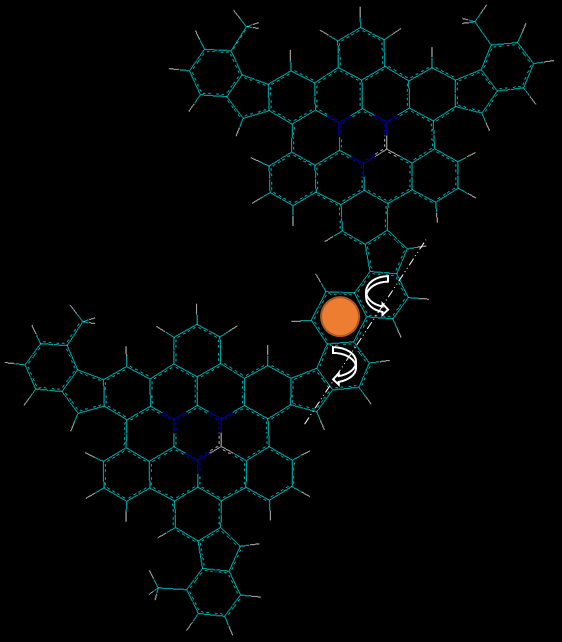
\includegraphics[height=0.35\textwidth]{./images/Closed-ring-dimer-2}
	\label{fig:HBBNC-Closed-ring-dimer-2}
	}
	\caption{Same bond formation (methyl groups create new carbon rings with adjacent methyl-phenyl rings) for \subref{fig:HBBNC-AM1-methyl-groups-fuse-link-2-split hydrogen} pristine HBBNC and its ring closure counterpart.
		\subref{fig:HBBNC-Closed-ring-dimer-1},\subref{fig:HBBNC-Closed-ring-dimer-2}. 
	\subref{fig:HBBNC-Closed-ring-dimer-1} Two legs with the same turn direction connect and result in a straight line between newly formed ring and the already present phenyl legs.
		\subref{fig:HBBNC-Closed-ring-dimer-2} Two opposite turn directions are linked in the same bond type but the new formed ring does not lie on the connection line between legs.
	 Compared to the previously derived connection between unaltered molecules, the connection for ring-closure molecules is formed at an different angle to the molecular backbone and may help identify the type of bond.
	}
	\label{fig:HBBNC-ring-closure-motifs}
\end{figure}

\begin{figure}[] \centering
	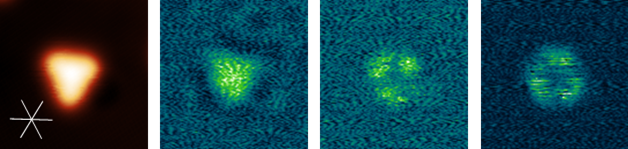
\includegraphics[width=0.7\textwidth]{./images/hbbnc-maps}
	\caption{STM Topography image and dI/dV maps for chosen energies. Choosing the spectroscopy energy to match one of the spectral maxima of the line spectra reveals the spatial distribution of electronic states as shown by the maps. While at 650 meV only the core contributes to the DOS, energies of 1200 meV and 1600 meV are located on the leg and edge positions respectively.}
	\label{fig:HBBNC-Ag111-dIdV-maps}
\end{figure}

\begin{figure}[] \centering
	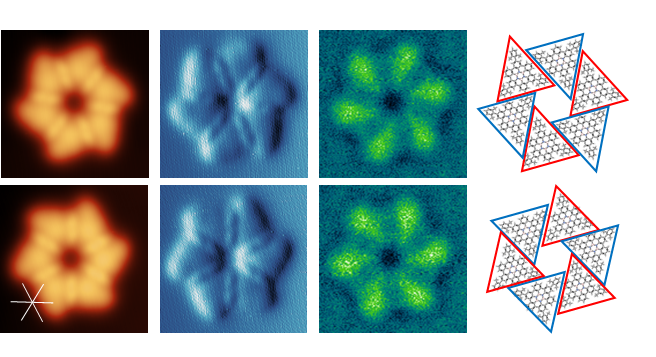
\includegraphics[width=0.7\textwidth]{./images/hbbnc-maps2}
	\caption{Comparison of two hexamers. While in STM the most apparent change is the orientation of the hexamer and the change in the star shaped protrusion, dI/dV maps (\SI{600}{\milli \eV}) emphasize the turn direction of the hexamer and its mirror image.}
	\label{}
\end{figure}

%\begin{figure}[] \centering
%	\includegraphics[width=0.7\textwidth]{./images/hbbnc-hexamer-afm}
%	\caption{Structure of an hexamer formed on Ag(111) after RT adsorption of a sub-ML of HBBNC. Sample was anealed to \SI{420}{\celsius} beforehand.}
%	\label{}
%\end{figure}

\begin{figure}[] \centering
	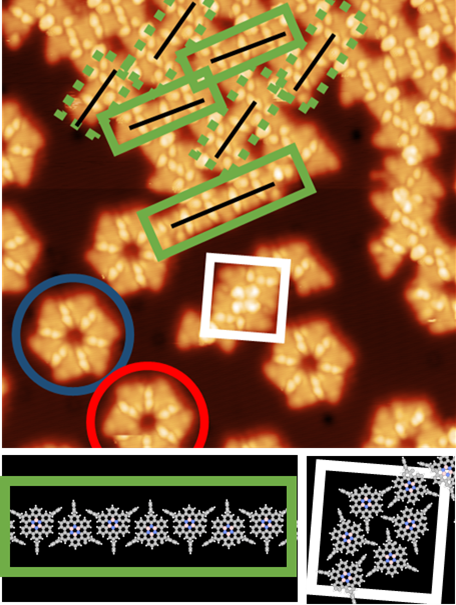
\includegraphics[width=0.7\textwidth]{./images/hbbnc-ag-111-rt-med-coverage-3}
	\caption{Medium coverage adsorption of HBBNC at RT on Ag(111). While the chiral assemblies are still present (blue/red circles), additional binding motifs like chains (green boxes) occur. Square  binding motifs are less frequent (white box). Imaging parameter: \SI{22.1}{\nano \meter}, \SI{2}{\volt}, \SI{0.4}{\nano \ampere}, Color scale: \SIrange{0}{400}{\pico \meter}.}
	\label{fig:HBBNC-medium-coverage-different-motifs}
\end{figure}

\begin{figure}[] \centering
	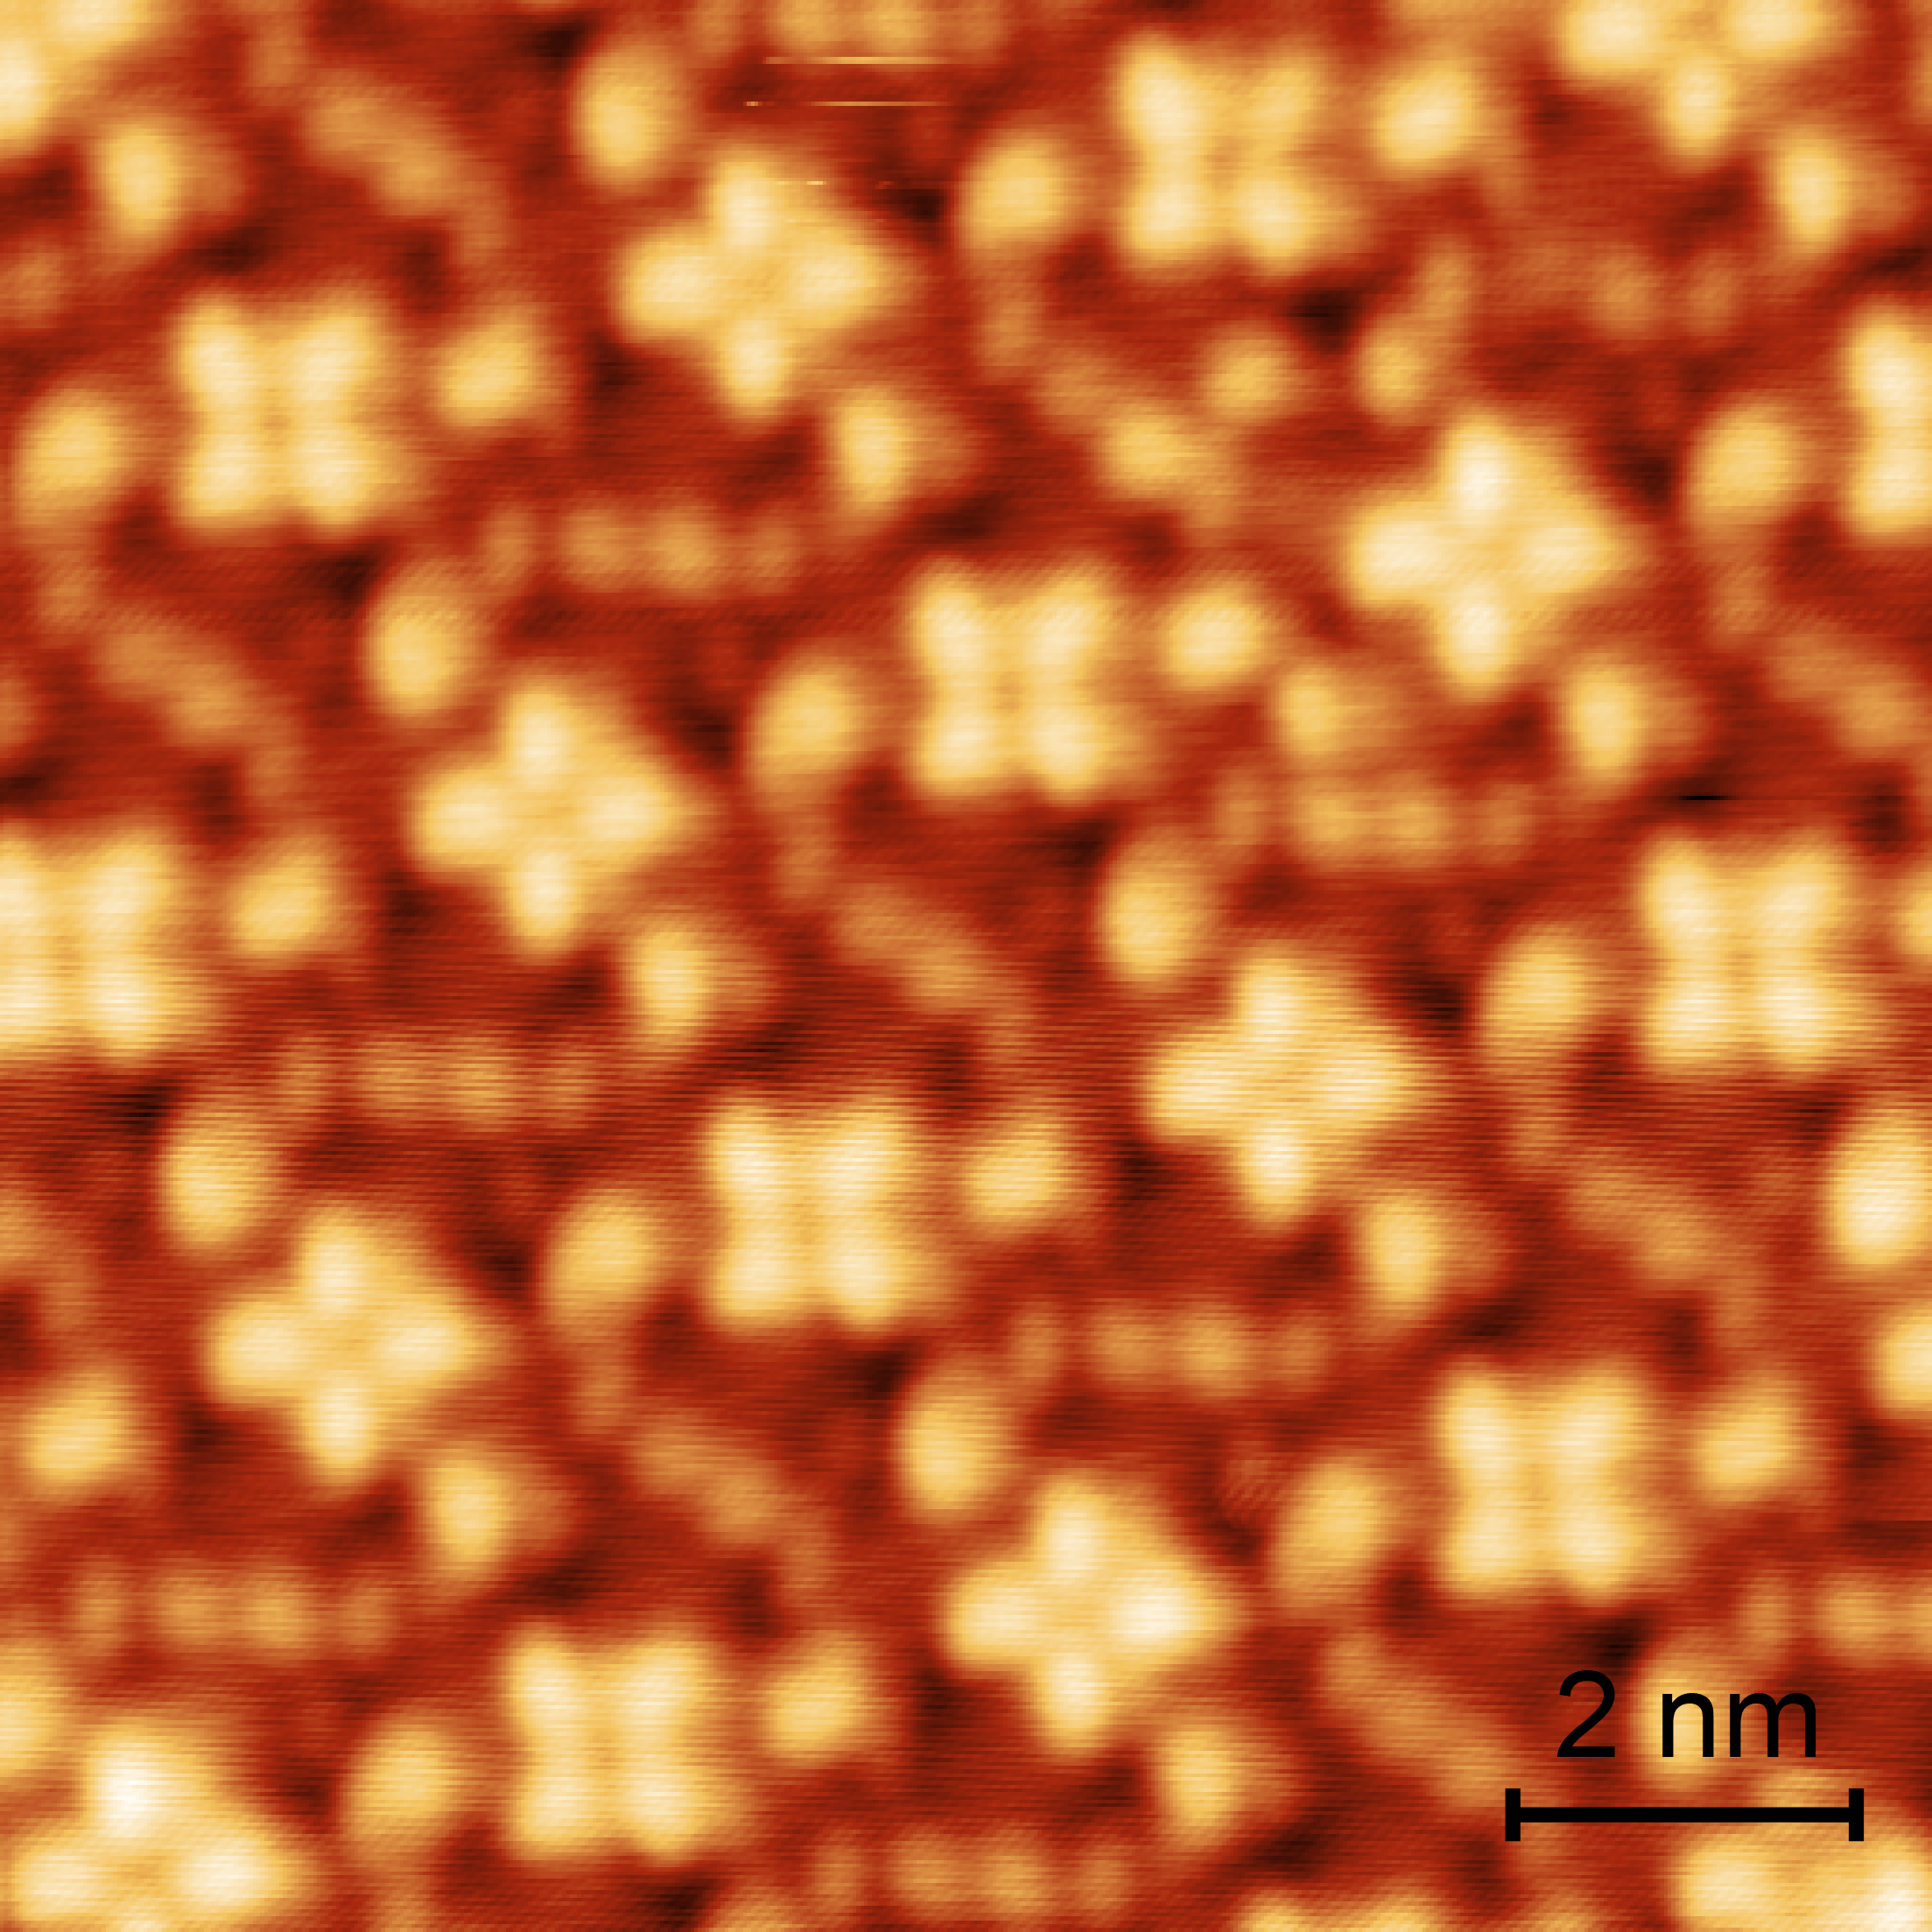
\includegraphics[width=0.35\textwidth]{./images/A180515-095412}
	\caption{STM topography image for high coverage adsorption of HBBNC at RT on Ag(111). The dominating pattern is the clover-leaf resembling the one observed for medium coverage. It is present here in two different orientations and distributed such that neighboring squares do not show the same orientation. Two squares with the same orientation are separated by lines made up of four bright spots aligned parallel to the square edge and diagonal. Squares with different rotations show a single protrusion with larger apparent height. Imaging parameter: \SI{11.07}{\nano \meter}, \SI{-250}{\milli \volt}, \SI{0.2}{\nano \ampere}.}
	\label{fig:HBBNC-high-coverage}
\end{figure}

%\begin{figure}[] \centering
%	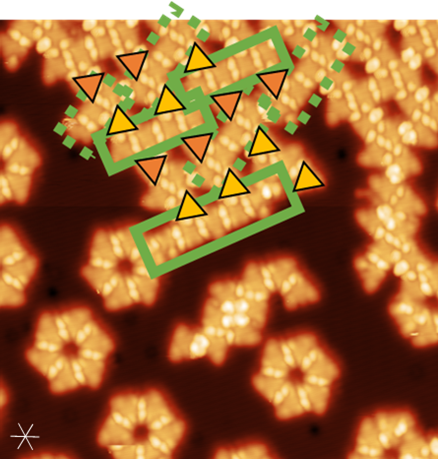
\includegraphics[width=0.7\textwidth]{./images/hbbnc-ag-111-rt-med-coverage-spacer-mol}
%	\caption{Rows are separated by two sets of spacer molecules (orange/yellow). 
%		\textcolor{red}{\textbf{What is their position in the unit cell? Rotation? Separation to all the other molecules?}}
%	}
%	\label{}
%\end{figure}

\begin{figure}[] \centering
	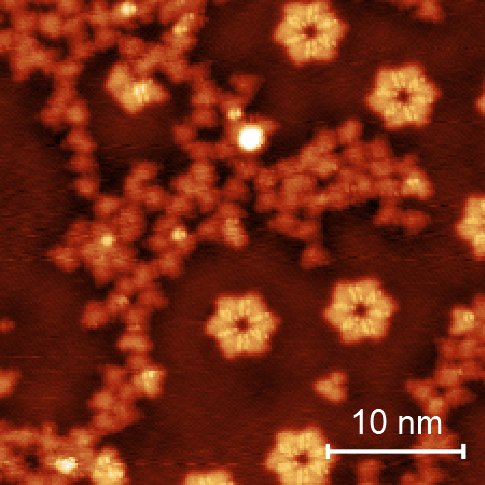
\includegraphics[width=0.35\textwidth]{./images/00239-180605-STM}
	\caption{STM topography image for a RT preparation of HBBNC on Ag(111) that is annealed to \SI{420}{\celsius}. After cooling down to RT, additional HBBNC molecules are deposited and the sample is investigated at $l_{He}$ temperatures. The sample shows both typical features pressent for an annealed sample (percolated network formation) and RT assembly (hexamers). Imaging parameter: \SI{35}{\nano \meter}, \SI{-70}{\milli \volt}, \SI{5}{\pico \ampere}., Color scale \SIrange{0}{250}{\pico \meter}}
	\label{fig:HBBNC-anneal-RT}
\end{figure}